\chapter{Evaluating the impact of quality score calibration on variant calling}
\label{ch:evaluating}
\section{Introduction}

DNA sequencing is a powerful tool applied in many fields of biology. Understanding how DNA and changes in DNA influence organisms and how they interact with their environment is a fundamental goal of genetics. Correctly identifying the composition of a sampled DNA molecule is therefore an important first step for many genetic studies. However, this task is not trivial; sequencing technology is inherently prone to errors which can make it difficult to discern true biological effects from technical errors \parencite{fox_accuracy_2014, wu_estimating_2017}. 

Because of this error, the same piece of DNA is usually sequenced multiple times to attempt to get multiple measurements and a model is applied to infer the sample genotype \parencite{li_statistical_2011, garrison_haplotype-based_2012, poplin_scaling_2018}. While a few sequencing errors do not impede accurate inference of the genotype of a monoploid sample, sequencing errors can be difficult to distinguish from heterozygosity in diploid organisms. This problem is even more difficult for samples with higher ploidy. However, using a statistical model enables a systematic approach to genotyping every site in the genome.

Additionally, a model allows the incorporation of auxiliary information when deciding the genotype at a site in a sample. For example, variant calling models often incorporate population genetic parameters that can help distinguish between sequencing errors and biological variation. The expected heterozygosity parameter \theta{} is particularly important; it usually parameterizes some prior on the probability of a base matching the reference genome. If this deviates significantly from the true value, the model may mistakenly classify truly heterozygous sites as errors or vice versa.

The goal of using a model to call variants is to integrate a wide variety of information to make a principled decision about whether or not a variant exists. An important source of information on the trustworthiness of each sequenced base is the base quality score \parencite{ewing_base-calling_1998, ewing_base-calling_1998-1}. This is a score, usually between 2 and 43, that encodes the probability the sequence is an error in the Phred scale. That is, the score $Q = -10\log_{10}P(\text{Base is an error})$. This number is then rounded to the nearest integer and encoded as a character, shifted by 33, in the sequencing data.

Since these numbers can vary significantly in the same line with few patterns, quality scores can't usually be compressed very well by common compression algorithms. That gives sequencing data large file sizes that make it expensive to store the data for a lengthy period of time. Thus, these quality scores are often binned to reduce the amount of variation in the scores, enabling improved compression \parencite{shibuya_better_2019, malysa_qvz_2015, yu_quality_2015, noauthor_reducing_2014}. Most binning methods attempt to do so in a way that minimizes the difference between the error rate of the bin and the error rate the bin should have according to its assigned score. However, there can still be a disconnect between the predicted error rate and the actual error rate. Furthermore, as the resolution of quality scores is reduced, some information about the true score at each base is lost. Interestingly, \textcite{yu_quality_2015} find that compressing scores by removing quality scores from all sites that are not likely to vary based on the k-mer composition of the data, but keeping quality scores intact at sites that may contain errors or true variants increases the quality of output genotype calls.

To restore quality score resolution before analysis and to ensure quality scores accurately reflect the probability of error at every base, a process known as base quality score recalibration (BQSR) is sometimes performed \parencite{auwera_fastq_2013, pfeifer_next-generation_2017}. This attempts to use known information about sequencing errors to calibrate the quality scores. The most common method for doing so implemented in the Genome Analysis Toolkit (GATK) requires aligned reads and a set of variable sites that are removed from analysis. The algorithm then looks for bases that do not match the reference, assumes they are errors, and uses those errors to recalibrate the quality scores. See Chapter \ref{ch:kbbq} for more information on quality scores and base quality score recalibration.
	
The ultimate goal of quality scores and base quality score recalibration is to make it easier to identify erroneous bases, which should improve the set of variants a variant caller emits. However, evidence supporting the use of base quality score recalibration is limited and whether base quality score recalibration is worthwhile is subject to debate. The procedure has aided in detecting rare variants \parencite{ni_improvement_2016}, and a recalibration procedure that integrates mapping errors into quality scores seems to improve variant detection \parencite{li_improving_2011}. The goal of this chapter is to investigate the degree that base quality score recalibration affects variant calling to enable informed decisions for constructing variant calling pipelines, especially for non-model organisms.

\section{Methods}

% Subsampling of database of variable sites - move this to Ch5
In order to determine how misspecification of the database of variable sites affects the calibration of GATK's BQSR procedure \parencite{auwera_fastq_2013}, I simulated datasets with various levels of false negative and false positive variants. In this case, false negative variants in the database of variable sites causes a site that should be ignored to not be ignored, greatly increasing the number of bases that GATK classifies as sequencing errors. On the other hand, false positive variants remove a site from GATK classification, so the effect is likely to be small except for large false positive rates.

To create each simulated dataset, I began with the high coverage synthetic diploid dataset described in \textcite{li_synthetic-diploid_2018} with reads aligned to hg19. This dataset was constructed by mixing DNA from the CHM1 and CHM13 hydatidiform mole cell lines to create a synthetic diploid sample. It includes a VCF of variant calls and a BED file representing regions where the authors are confident the calls in the VCF are correct. I subset the full dataset to only reads aligned on Chromosome 1 and overlapping the BED of confident regions using the samtools view command \parencite{li_sequence_2009} and the -L parameter. I then used the samtools (version 1.10) view command with the -F 3844 flag to remove unmapped, secondary, and supplementary alignments as well as reads marked as failing quality checks and as PCR duplicates. I then used the fixmate and view commands with flag -f 1 to remove any singleton reads.

To create each false negative dataset, an appropriate number of sites from the VCF were randomly sampled with BCFTools (version 1.10.2) and the shuf (version 8.32) program. To create each false positive dataset, all sites from the VCF were extracted in BED format with the BCFTools query command, then subtracted from the BED of confident regions with bedtools (version v2.27.1) subtract \parencite{quinlan_bedtools_2010}. The appropriate number of sites were then sampled with the shuf program and appended to the sites from the VCF to generate the BED file of all sites to exclude. Thus, I created variable site sets that were artificially crafted to have different rates of false positive and false negative calls, from 0 to 100 in steps of 20.
These files were then provided as input to the GATK (version v4.1.8.0-5-g1836ab0-SNAPSHOT) BaseRecalibrator tool and calibration was evaluated with GATK's AnalyzeCovariates tool.

As a control, I compared each result to the raw, uncalibrated data. To see how a reference-free recalibration method affected variant calling, I also recalibrated the data with KBBQ (commit ID 9167b72599892a33493d8ebdc01fac33990c1738), with the options -\phantom{}-genomesize 214206308 and -a .15 .

I then called variants on each dataset using GATK HaplotypeCaller \parencite{poplin_scaling_2018}. The false positive rate of 100\% produced no output calls except in the case of 0\% false negative rate, which produced fewer calls than any other set. All datasets containing a 100\% false positive rate were therefore discarded. I evaluated these output SNP calls using RealTimeGenomics' RTG Tools (version 39691f9f) vcfeval program \parencite{cleary_comparing_2015} and the confident region set along with the confident call set. I first ran the tool using the default settings, which also produces a ROC curve for the calls' GQ annotation. I also ran the tool using the -\phantom{}-vcf-score-field=QUAL option, which produces ROC curves for the site's QUAL annotation. This enabled comparison of the sensitivity and false positive rate trade-off of the two scores for each dataset. These two annotations were chosen because they represent an overall summary of the quality of the called variants.

The false positive rate for the ROC curves was found by dividing the number of false positive calls in each dataset at each value of QUAL or GC and below by the number of true negative sites. The number of true negative sites was obtained by subtracting each true positive variant from the BED file containing the confident regions of the callset. This rate had to be computed, as vcfeval does not report a false positive rate. As the RTG-tools manual states, the program doesn't try to compute the possible number of true negatives, as calls could in theory occupy many or no reference bases. However, as I analyze only SNP data here,  estimating the true number of negatives as the number of sites that are within the confident regions but outside variant sites specified by the truth set should be sufficient. The true positive rate was calculated by taking the number of true positive calls in each dataset for each value of QUAL or GC and dividing by the number of positive calls in the truth set, as reported by the vcfeval output.

To evaluate the output calls, I plotted the number of false positive and true positive SNP calls for each dataset. I also constructed a heat map showing the F-statistic of each dataset. This is the harmonic mean of the sensitivity and precision of the calls and is one way to summarize the accuracy of the calls. All plots and heatmaps were made using R \parencite{r_core_2020} and ggplot2 \parencite{wickham_ggplot2_2016} using the viridis color palette \parencite{garnier_viridis_2018} and the Okabe-Ito palette implemented in colorblindr to ensure the plots remain interpretable by those with colorblindness and after photocopying.

%Filter info + justifications:
%#filter: only snps
%#filter: DP > 35 & DP < 65 (+-2 SDEV from mean of ~50 assuming poisson)
%#filter: QUAL > 75; this is ~bottom 1% and the maximum F
%#   value from the previous analysis is between 75 and 150.
To see how filtering the calls affected their quality, I then identically filtered each variant set with two filters using bcftools view \parencite{li_sequence_2009}. The first filter is a depth filter, only accepting variants that have more than 35 aligned reads and fewer than 65. This is within two standard deviations of the mean sequencing depth of \~50, assuming the read depths are Poisson distributed. The second filter is a QUAL filter, accepting only calls with a QUAL of over 75. This threshold was chosen because it is approximately the bottom 1\% of QUAL values in each dataset and it is the lowest QUAL value that maximizes the F-statistic of all the datasets. I then calculated the same statistics and made the same plots using the filtered calls.

%THE STORY IS COMING TOGETHER: The range in number of TP calls grows after filtering! Prior to filtering there is a big difference in the number of FPs in each dataset (1009), but this difference shrinks after filtering to 548. The difference in number of true positives starts at 240, but grows to 2044 after filtering.


%Simulated reads
%
In order to investigate how calibration affected variant calling performance on a medium-coverage dataset from a highly heterozygous sample with a low-quality reference, as might be the case when sequencing a non-model organism, I created a simulated dataset. I first randomly sampled contigs from the first release of the \textit{Eucalyptus grandis} reference (SRA accession AUSX00000000.1) until I sampled 5 million base-pairs, which at 20X coverage for a diploid genome would yield approximately 200 million base-pairs of synthetic sequence data. I then simulated heterozygous sites in the genome with simuG (version v1.0.0) \parencite{yue_simug_2019} with a transition/transversion ratio of 2 and 125,000 SNPs to emulate the conditions observed in eucalypts \parencite{kulheim_comparative_2009}. I concatenated the subsampled and simulated genomes to create a diploid reference and simulated reads from it using ART (version MountRainier-2016-06-05; \cite{huang_art_2012}). I simulated 101-bp long reads with a mean fragment length of 300 and standard deviation of 20, with 20X coverage. I then aligned the simulated reads to the genome with NextGenMap version 0.5.2 \parencite{sedlazeck_nextgenmap_2013} and recalibrated the data 3 ways: 1) with GATK using the true set of heterozygous sites as the database of variable sites, 2) with GATK using a set of variant calls generated with HaplotypeCaller with the \texttt{-\phantom{}-stand-call-conf} set to 50 as the database of variable sites, and 3) using KBBQ (see Chapter \ref{ch:kbbq}) with the genome size parameter set to 5 million.

Including the simulator-assigned raw scores, this yielded four datasets with different quality scores to call variants with and compare the results. HaplotypeCaller was used on each dataset and given the subsampled genome as a reference and called with the \texttt{-\phantom{}-heterozygosity 0.025} option to represent the approximate heterozygosity of the data. As simuG doesn't output sample genotypes and the simulated sample is heterozygous at every site in the truth VCF, a sample column was added and the genotype of the sample at every site set to be 0|1 using sed. This VCF was then used as the truth comparison for rtg-tools vcfeval command and used to evaluate each set of variant calls. vcfeval was run in annotate mode and the output parsed using hapdip.js (version r66; \cite{li_toward_2014}) to generate summaries of each callset. Finally, vcfeval was also run in roc-only mode, once with the \verb|--vcf-score-field| set to GQ and once set to QUAL to produce ROC curves for each of these scores. The false negative rate was obtained by dividing the number of output false negatives by the length of the genome minus the number of simulated heterozygous sites.

% /storage/2017-03-15-eucalyptus/2020-09-28-kbbqflt
Finally, I ran KBBQ with the specified genome size 605951511 and coverage 240 to recalibrate a set of reads sequenced from an individual of the non-model species \textit{Eucalyptus melliodora} \parencite{orr_phylogenomic_2020}. This dataset contains reads from 3 leaves each from 8 branches, each leaf sequenced to a depth of approximately 10X. I then called variants using HaplotypeCaller and filtered the calls using the same filters from \textcite{orr_phylogenomic_2020}. I use BCFTools view to record the number of variable sites that were also recorded in the previously identified set of calls found using DeNovoGear \parencite{ramu_denovogear_2013}. I then compared these values to those found using the raw, uncalibrated reads and those found using the GATK recalibrated reads in \textcite{orr_phylogenomic_2020}.

Scripts to reproduce these analyses are included in Appendix \ref{ch:evaluating_code}.

\section{Results}
% Hapdip Analysis
To identify how errors in the database of variable sites affects variant calling, I simulated different datasets with known false positive rates, plotted the calibration and calculated the root mean squared error (RMSE) of the data recalibrated with the model trained using each database as the known sites input to GATK BaseRecalibrator. These plots are shown in figure \ref{figure:fpr}, and the RMSE of the quality score for each dataset is shown in table \ref{table:fpr}. For all these datasets, the false negative rate is 0. As the false positive rate increases, the degree of miscalibration doesn't change significantly except for the 100\% false positive rate dataset, which is very poorly calibrated; however, this calibration is likely an artifact (see section \ref{sec:kbbq_discussion}).

\begin{figure}
\centering
	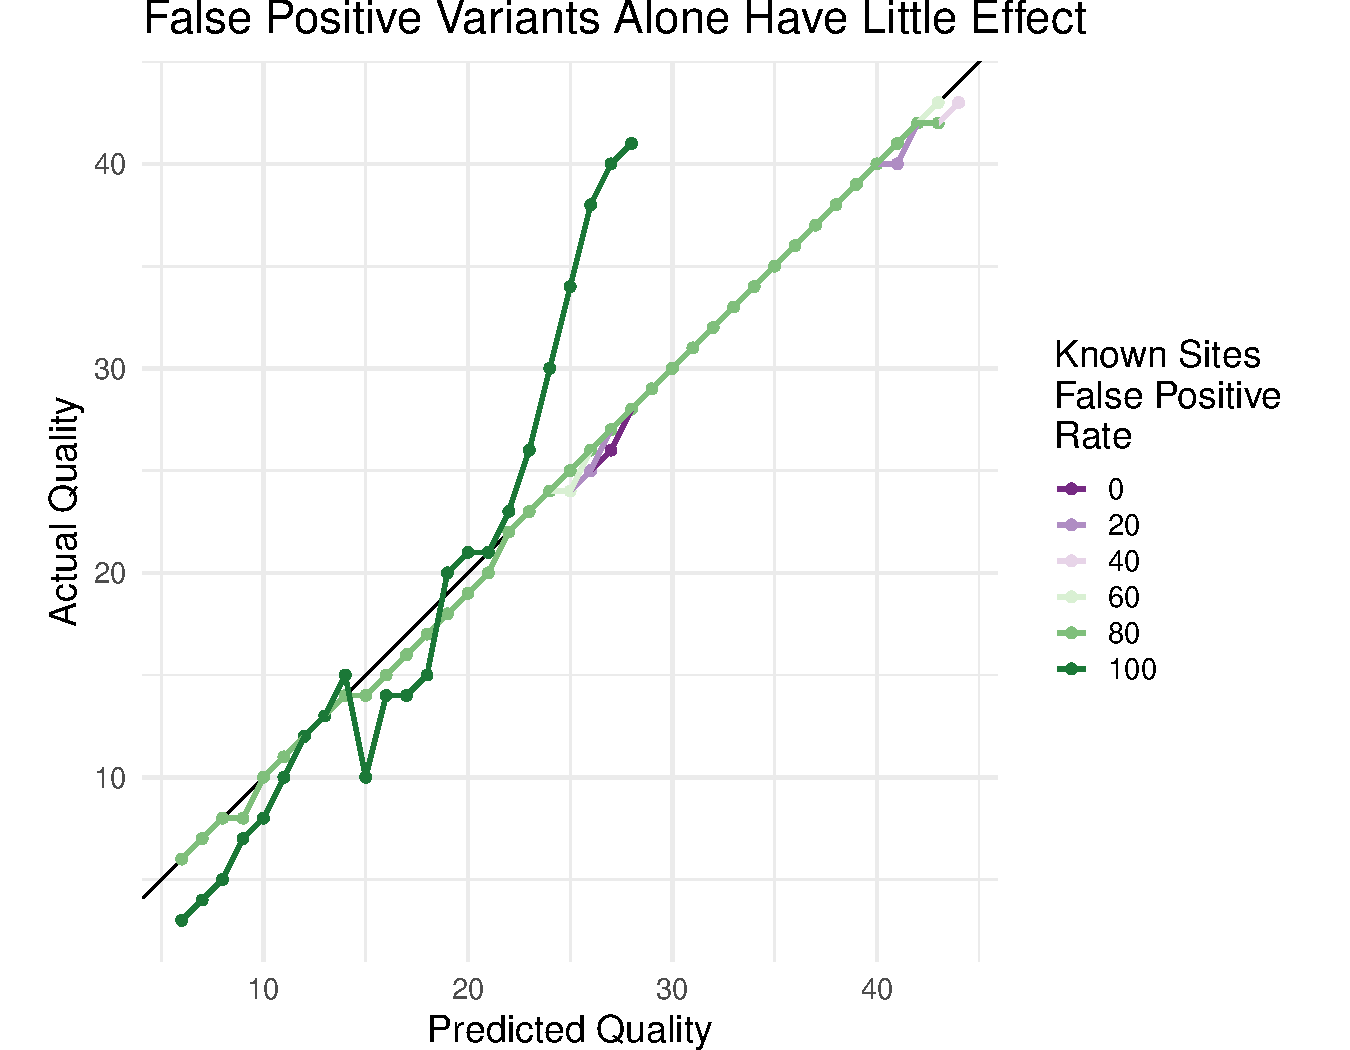
\includegraphics[width = .6\textwidth]{fpr.pdf}
	\titlecaption{False Positive Only Calibration}{Base quality score calibration for a range of false positives in the database of variable sites. The false negative rate for all datasets is zero. Increasing the false positive rate does not significantly impact the quality of the calibration. The poor calibration at a 100\% false positive rate is likely an artifact (see Section \ref{sec:kbbq_discussion}).}
	\label{figure:fpr}
\end{figure}

\begin{table}
\centering
\begin{tabular}{r l}
\toprule
False Positive Rate & RMSE \\
\midrule
0 & 0.60 \\
20 & 0.58 \\
40 & 0.53 \\
60 & 0.49 \\
80 & 0.49 \\
100 & 5.50 \\
\bottomrule
\end{tabular}
\titlecaption{False Positive Calibration Errors}{The root mean squared error of quality score for reads recalibrated using a database of variable sites with different false positive rates. The false negative rate for each dataset is 0\%.}
\label{table:fpr}
\end{table}

I also simulated different databases of variable sites with differing false negative rates and similarly used it to recalibrate the CHM1-CHM13 data. In these datasets, the false positive rate is 0\%. The plotted calibration and RMSE of the recalibrated data is shown in figure \ref{figure:fnr} and table \ref{table:fnr}. As the false negative rate increases, the degree of miscalibration also steadily increases.

\begin{figure}
	\centering
	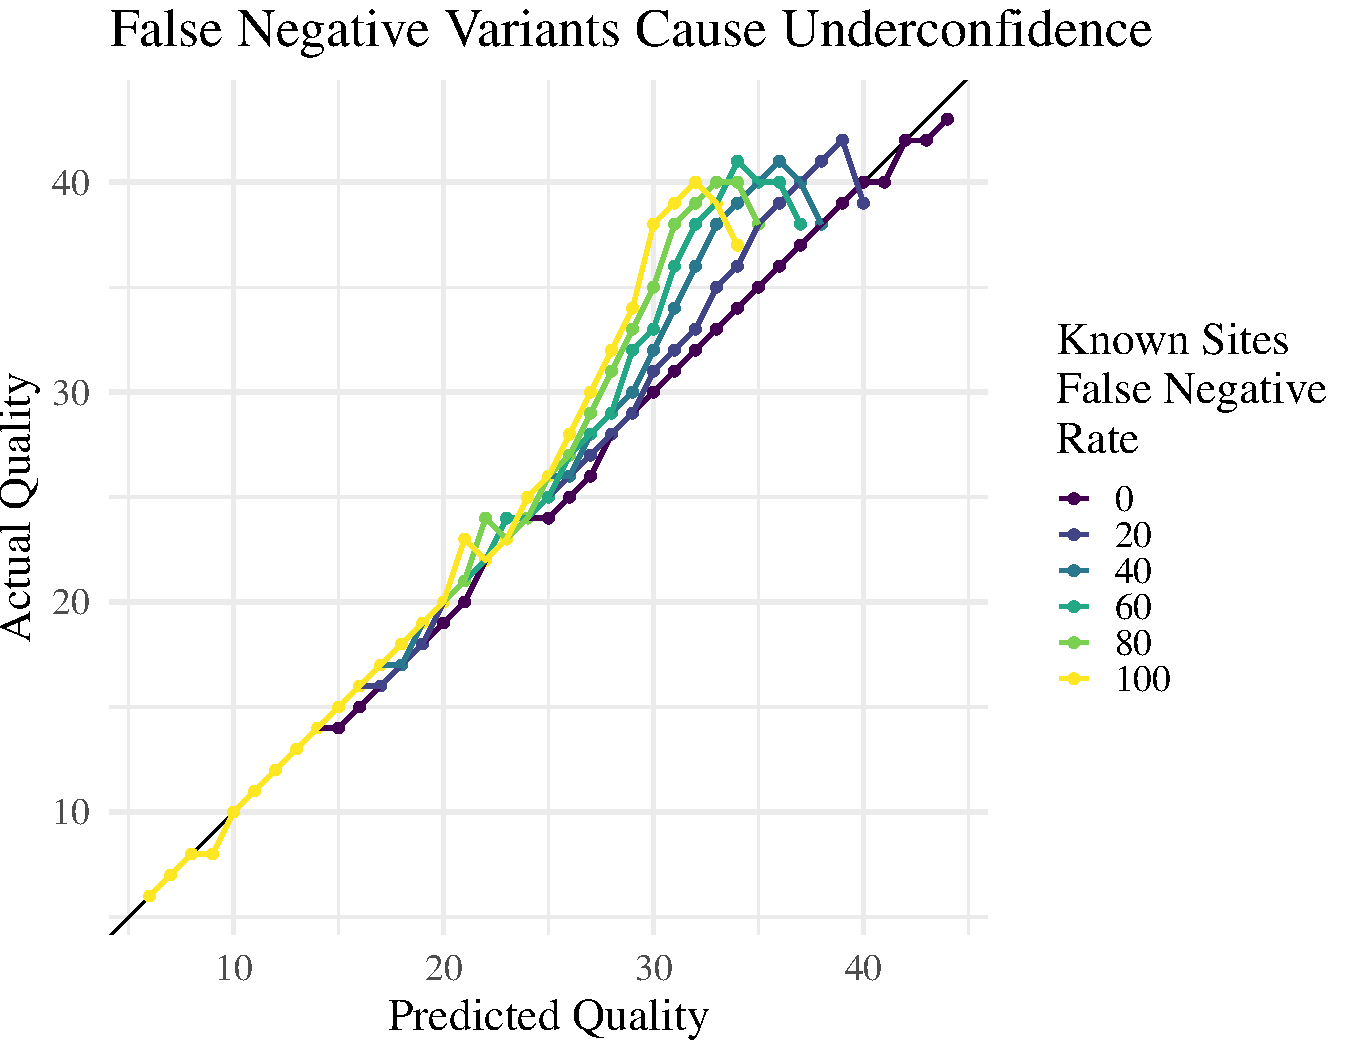
\includegraphics[width=.6\textwidth]{fnr.pdf}
	\titlecaption{False Negative Only Calibration}{Base quality score calibration for a range of false negatives in the database of variable sites. The false positive rate for all datasets is zero. Increasing the false negative rate significantly decreases the quality of the calibration, causing increasing  underconfidence in quality scores as the false negative rate rises.}
	\label{figure:fnr}
\end{figure}

\begin{table}
\centering
\begin{tabular}{r l}
\toprule
False Negative Rate & RMSE \\
\midrule
0 & 0.60 \\
20 & 1.32 \\
40 & 2.10 \\
60 & 2.57 \\
80 & 2.90 \\
100 & 3.20 \\
\bottomrule
\end{tabular}
\titlecaption{False Negative Calibration Errors}{Root mean squared error of quality score for reads recalibrated with a database of variable sites simulated with the given false negative rate. The false positive rate for each dataset is 0\%.}
\label{table:fnr}
\end{table}

To see if there were any interactive effects of false positive rate and false negative rate, I also simulated datasets with varying false positive and false negative rates. The RMSE of the calibrated scores is reported in Table \ref{table:fnrfpr} and summarized in Figure \ref{figure:fnrfpr}. These datasets were simulated separately from the above datasets, so there are slight differences in the calibration of the resulting reads.
As before, the number of false negatives significantly impacted calibration quality. In contrast to the false positive only dataset with a 0\% false negative rate, increasing the false positive rate also increased the amount of error in the calibration. Thus, false positives in the database of variable sites seem to enhance miscalibration caused by false negatives.

\begin{figure}
	\centering
	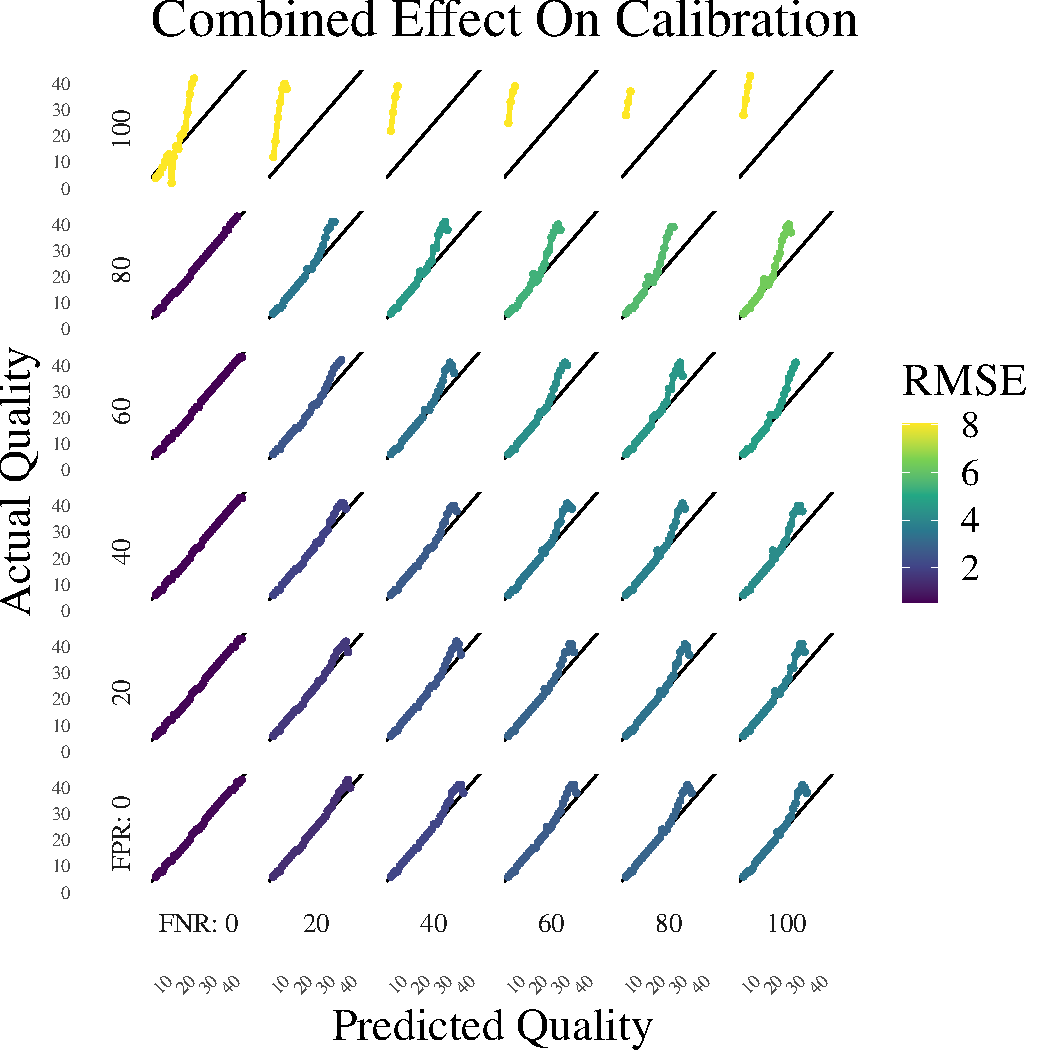
\includegraphics[width = \textwidth]{fnrfpr.pdf}
	\titlecaption{Combined Calibration}{Calibration of base quality scores of reads recalibrated using a database of variable sites with varying ranges of false negatives and false positives. The RMSE of the quality scores of the resulting calibration are used to color each line. Across the columns are each false negative rate, and each row represents a false positive rate. Except for at a false negative rate of 0, increasing either the false positive rate or the false negative rate increases the RMSE. See Table \ref{table:fnrfpr} for the RMSE values and the discussion in Section \ref{sec:kbbq_discussion} about false positive rates of 100\%}
	\label{figure:fnrfpr}
\end{figure}

\begin{figure}
	\centering
	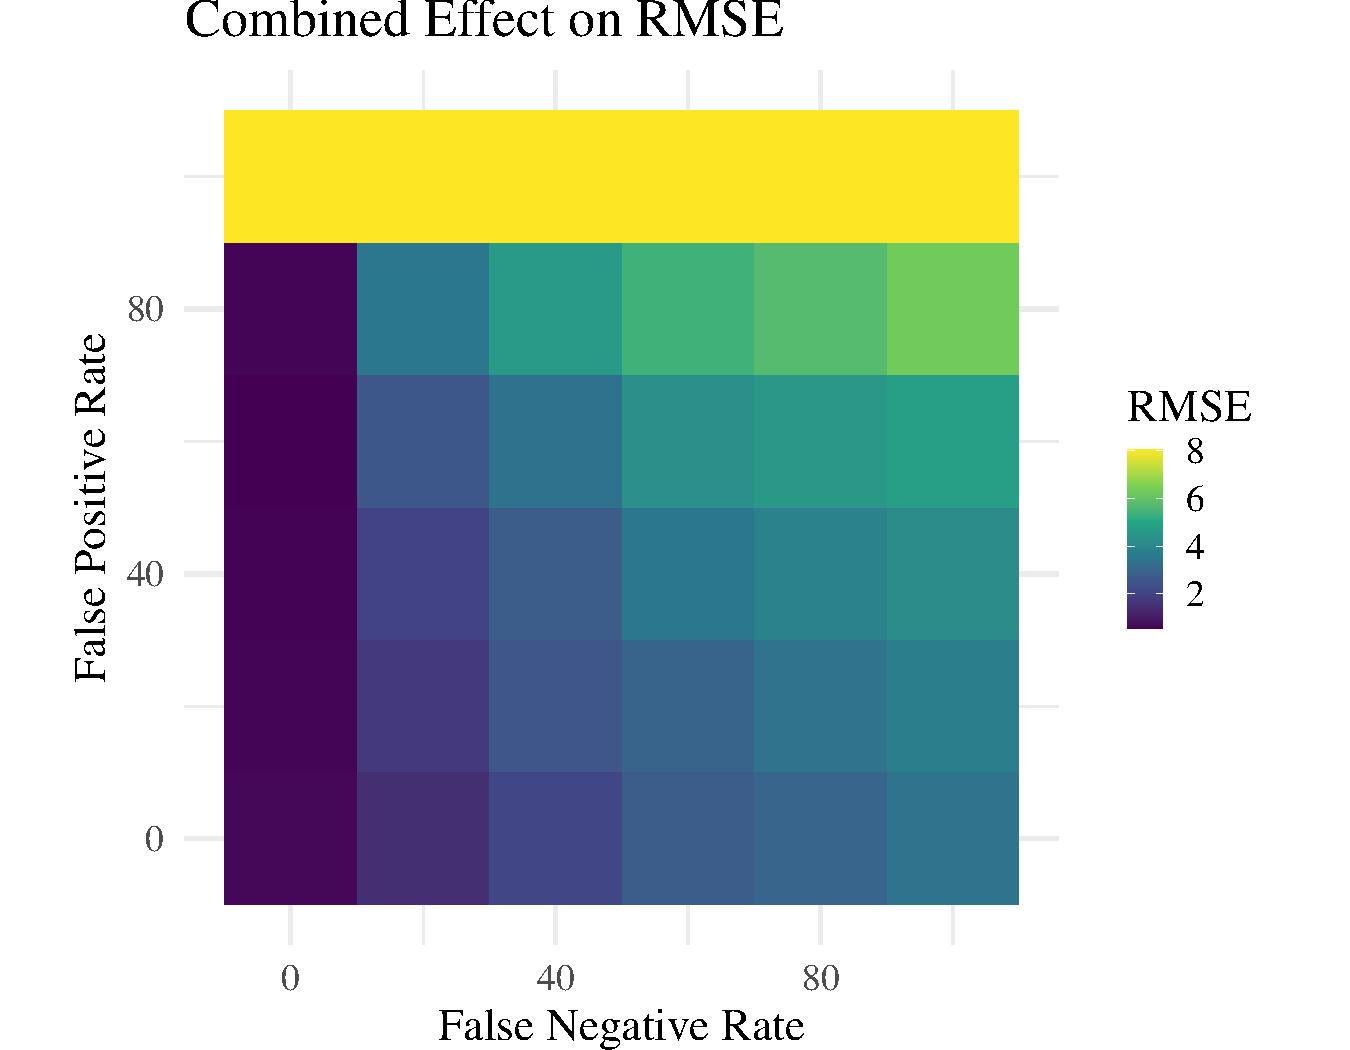
\includegraphics[width = .6\textwidth]{fnrfpr_heatmap.pdf}
	\titlecaption{Combined Calibration Heat Map}{Heat map of base quality calibration of varying ranges of false negatives and false positives. Databases of variable sites with differing false positive and false negative rates were constructed and the RMSE of the quality scores of the resulting calibration were calculated. Across the columns are each false negative rate, and each row represents a false positive rate. Except for at a false negative rate of 0, increasing either the false positive rate or the false negative rate increases the RMSE. See Table \ref{table:fnrfpr} for the RMSE values and the discussion in Section \ref{sec:kbbq_discussion} about false positive rates of 100\%}
	\label{figure:fnrfpr_heat}
\end{figure}

\begin{table}
\centering
\begin{tabularx}{.5\textwidth}{ l  X  X  X  X  X  X }
\toprule
\multirow{2}{*}{FPR} & \multicolumn{6}{c}{FNR} \\ \cmidrule(lr){2-7}
    & 0    &   20 &   40 &   60 &   80 &   100 \\
%&    &      &      &      &      &      & \\ %blank line
\midrule
0   & .641 & 1.45 & 2.08 & 2.73 & 2.99 & 3.38 \\
20  & .599 & 1.73 & 2.54 & 2.96 & 3.39 & 3.76 \\
40  & .555 & 2.02 & 2.71 & 3.50 & 3.84 & 4.16 \\
60  & .531 & 2.58 & 3.37 & 4.27 & 4.51 & 4.73 \\
80  & .593 & 3.52 & 4.62 & 5.38 & 5.73 & 6.32 \\
100 & 8.05 & 22.0 & 24.3 & 26.4 & 25.8 & 28.9 \\
\bottomrule
\end{tabularx}
\titlecaption{Combined Calibration Errors}{Root mean squared error of base quality score for data calibrated with databases of variable sites containing different levels of false positives and false negatives. The columns indicate false positive rates, the rows indicate false negative rates. The values in each cell are the RMSE of the quality scores for the reads recalibrated with the database of variable sites with false positive and false negative rate appropriate for its row and column. See Figure \ref{figure:fnrfpr_heat} for a graphical representation. The data in the 100\% false positive rows are likely artifacts; see section \ref{sec:kbbq_discussion} for more information.}
\label{table:fnrfpr}
\end{table}


% Variant Call Evaluation

To evaluate the output calls, I plotted the number of true positives and false positives for each dataset recalibrated using sets of variable sites with differing false negative and false negative rates (Figure \ref{fig:vc_fptp}). This shows that after recalibration, improved calibration increases the number of true positive variants called. However, improved calibration also increases the number of false positives. More detail about the relationship between false positives and negatives in the database of calibrated sites are shown in the heat maps in Figure \ref{fig:vc_p}. Interestingly, the raw uncalibrated data exhibited the most positive calls of any other callset.


\begin{figure}
\centering
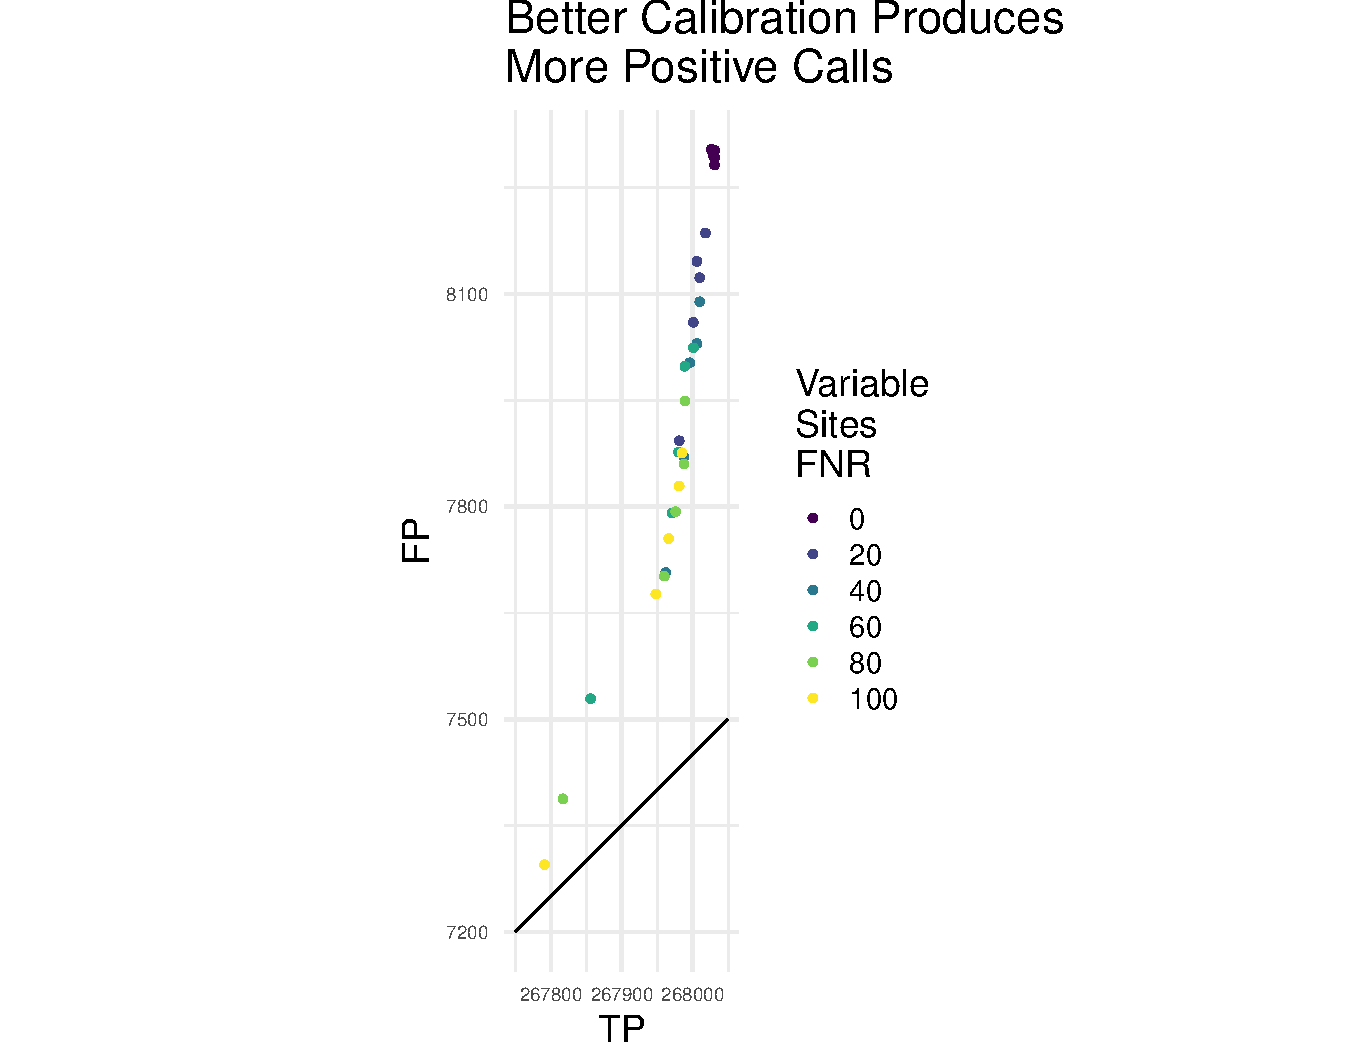
\includegraphics[width = .8\textwidth]{tp_fp_plot.pdf}
\titlecaption{More Accurate Known Sites Increases Number of Unfiltered Positive Calls}{The output number of positive calls for each dataset. The false negative rate of the set of variable sites used to calibrate the reads used to produce each callset is shown. As the false negative rate decreases, the number of both true positive and false positive calls increases. The raw, uncalibrated data exhibits the highest number of positive calls.}
\label{fig:vc_fptp}
\end{figure}

\begin{figure}
\centering
\includetwo{fp_heatmap.pdf}{tp_heatmap.pdf}
\titlecaption{Both False Negative and False Positive Rate Contribute to Increased Number of Unfiltered Positive Calls}{The output number of false positive calls for each dataset. The false negative and false positive rate of the set of variable sites used to calibrate the input reads or the name of the dataset for non-simulated datasets is shown on the X and Y axis. The color of each cell represents the number of unfiltered false positive (left) or true positive (right) SNP calls. As the false negative and positive rates of the database of variable sites decrease, the base quality scores become more calibrated, and more calibrated data produces more false positive and true positive calls. However, the raw data produces the most true positives and the most false positives.}
\label{fig:vc_p}
\end{figure}

To determine the impact of these variants on the overall quality of the callsets, I constructed heatmaps of the sensitivity and precision of each dataset (Figure \ref{fig:vc_sens_prech}). As the data become more well-calibrated, the sensitivity of the caller increases; however, the precision of the caller also decreases. This is also seen in the raw calibration: it has the highest sensitivity and lowest specificity of all the datasets. This means that the caller is able to detect more true variants, but a higher proportion of the calls it makes are false positives. To visualize the trade-off between sensitivity and precision, I plotted the precision against the sensitivity of each dataset, shown in Figure \ref{fig:vc_sens_prec}. To summarize the overall effect on accuracy, I show how the F-statistic changes across each dataset in Figure \ref{fig:vc_f_heatmap}. The callset made from the raw, uncalibrated data have the lowest F-statistic.

\begin{figure}
\centering
\includetwo{sensitivity.pdf}{precision.pdf}
\titlecaption{Better Calibration Increases Sensitivity and Reduces Precision}{The sensitivity (left) and precision (right) of the variant caller on each dataset with no filtering. As the base quality score calibration of the input reads increases, the sensitivity of the caller increases and the precision decreases. The data with raw quality scores has the highest sensitivity and lowest precision.}
\label{fig:vc_sens_prech}
\end{figure}

\begin{figure}
\centering
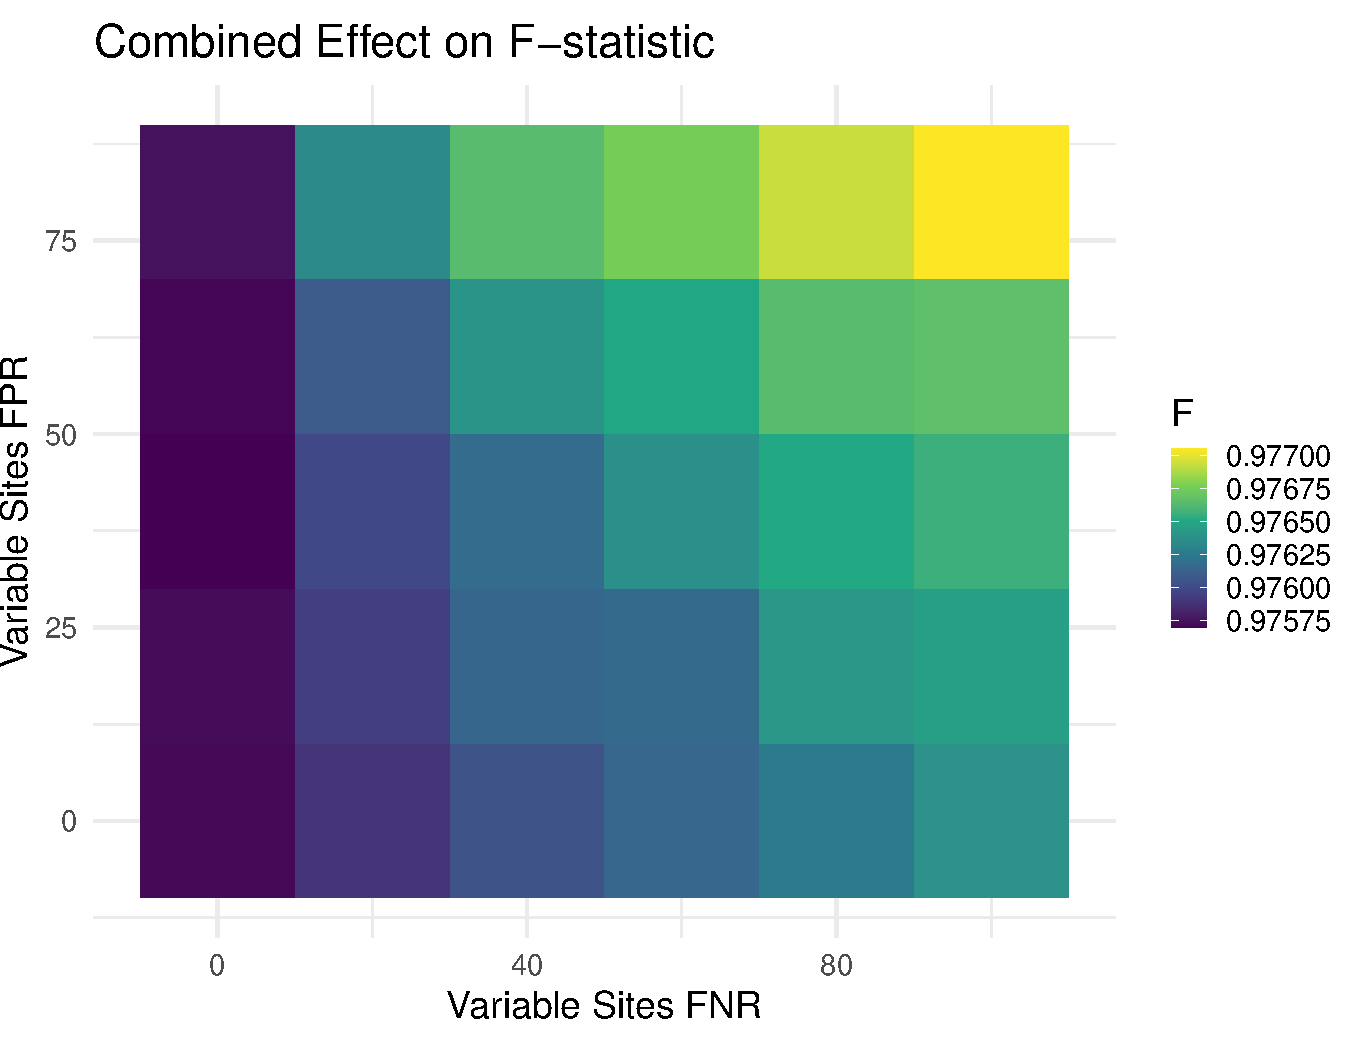
\includegraphics[width = .8\textwidth]{f_heatmap.pdf}
\titlecaption{F-statistic of Unfiltered Calls}{The F-statistic of the unfiltered calls of each dataset. As the base quality score calibration of the input reads increases, the F-statistic of the caller decreases. This is driven by the fact that the increase in sensitivity of the caller is much smaller than the decrease in precision. The raw, uncalibrated quality scores have the lowest F-statistic.}
\label{fig:vc_f_heatmap}
\end{figure}

Since the base quality score of the reads used to support each genotype call evidently plays a role in whether to emit a variant, I wanted to see how the differences in calibration affected the annotations output by the caller. To that end, I plotted a receiver operating characteristic (ROC) curve showing the trade-off between false positive and true positive rates for variants ordered according to their QUAL and GQ annotations (Figure \ref{fig:vc_rocs}). These are both statistics that summarize the quality of the emitted site in a single, increasing score, and so are well-suited for ROC analysis. According to the VCF standard, the QUAL score is a phred-scaled probability that the ALT allele(s) present in the call are not actually present, $P($ALT is wrong$)$. The GQ score is the phred-scaled conditional probability the genotype call is incorrect given the site is variable, $P($genotype is wrong $|$ site is variant$)$.

\begin{figure}
\centering
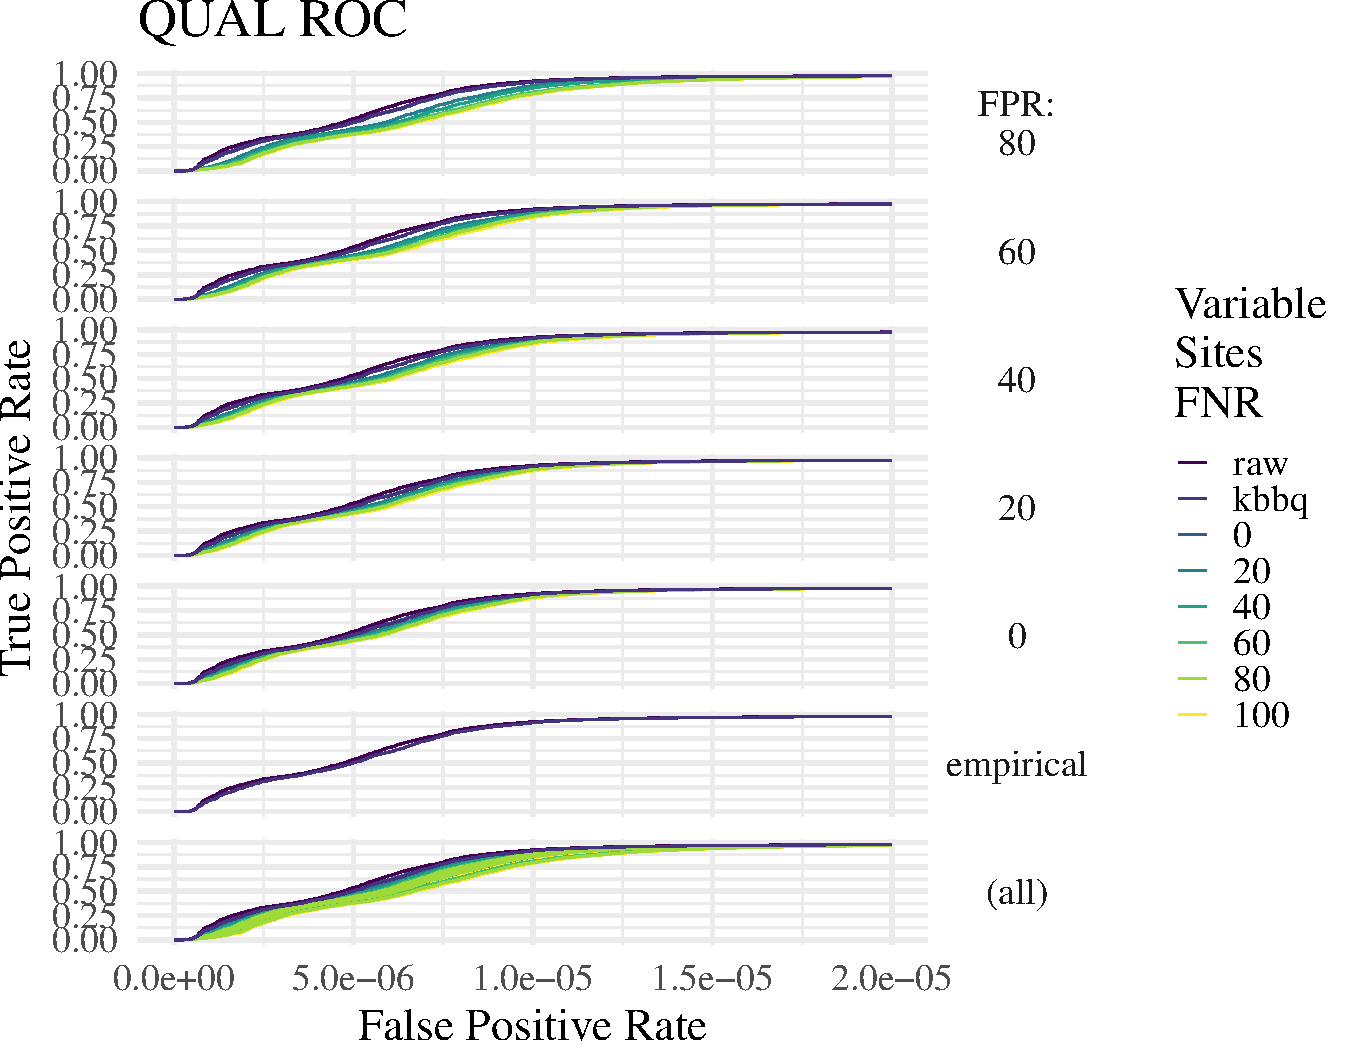
\includegraphics[width = .6\textwidth]{qualroc.pdf} \\
\vskip 1em
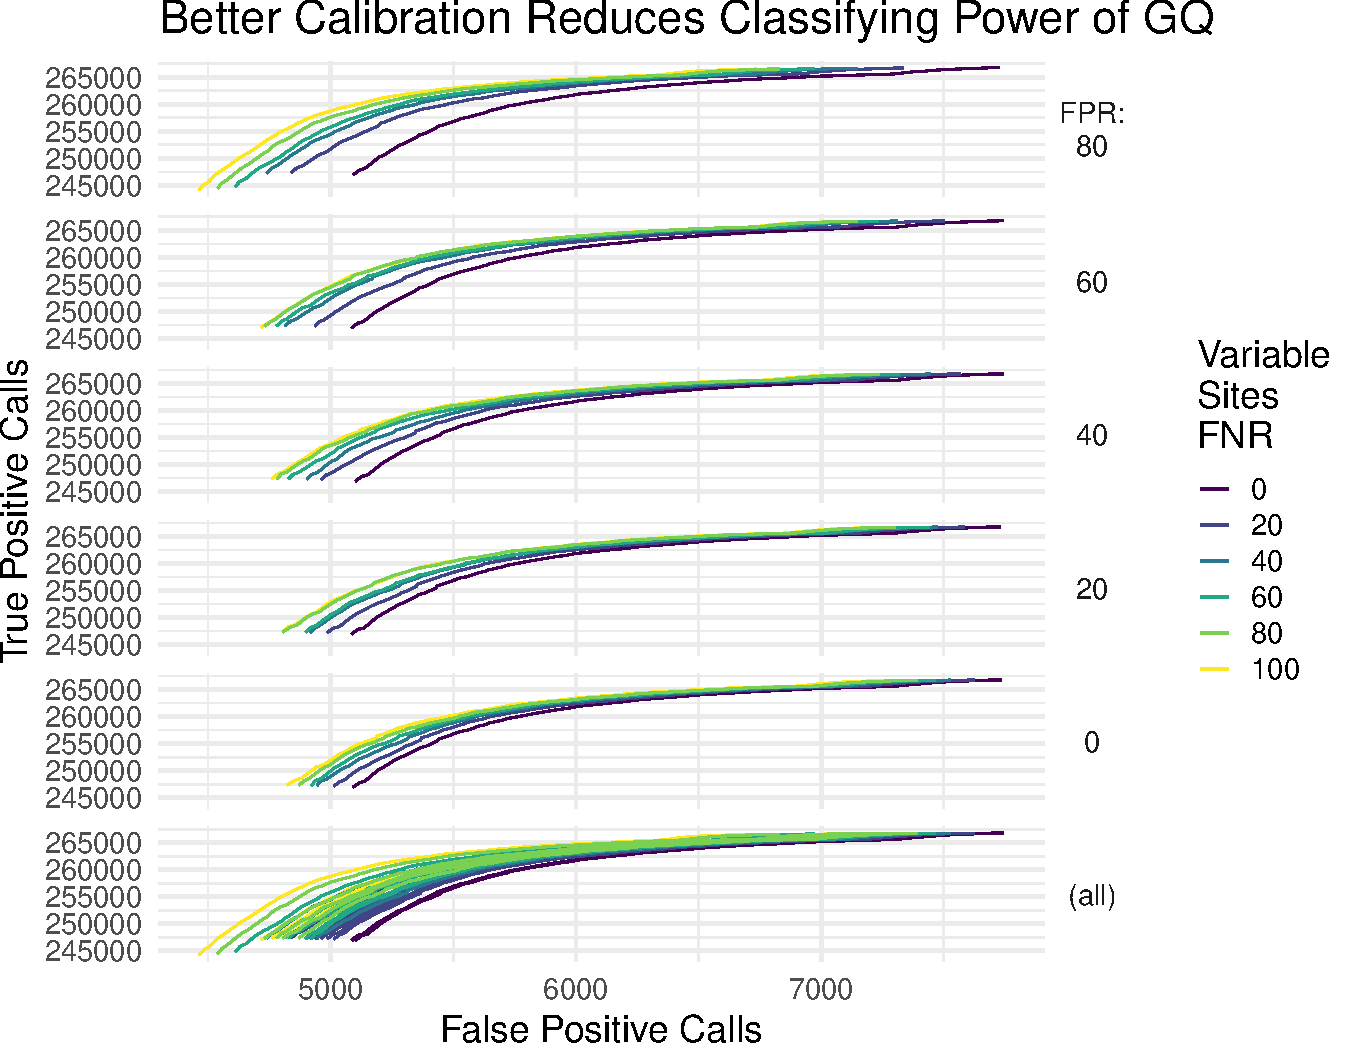
\includegraphics[width = .6\textwidth]{gqroc.pdf}
\titlecaption{Unfiltered ROC Curves}{The ROC curves for the QUAL (top) and GQ (bottom) score of an output call for the unfiltered calls of each dataset. The color of each line represents the false negative rate of the set of variant sites used as input to recalibrate the reads used to call variants. Each point in the line represents the number of false positive and false negative calls that have a score above the QUAL or GQ threshold for that point. As this threshold decreases, the number of false positives and true positives increases, though at different rates. These plots show that as the false positive rate increases, the number of true positive calls increases at a faster rate for the well-calibrated data than in other datasets for the QUAL classifier, but at a slower rate for the GQ classifier. The values for the two empirical datasets (raw and KBBQ), are shown on each plot. The other lines on each plot show values from calls made with reads that were recalibrated with variable site sets with the shown false positive rate.}
\label{fig:vc_rocs}
\end{figure}

As the ROC plots show that each dataset would respond to filtering differently, I examined how the calls would improve or not after filtration. I used a small QUAL filter filtering out variants with the lower 1\% of QUAL scores. This percentage coincides with the smallest QUAL value of the QUAL values that maximize the F-statistic of every dataset. These values are shown in Figure \ref{fig:vc_f_heatmap}. Depth filters are very common after variant calling, so I also used a depth filter to filter out calls that had unusually high or low depth.

% > rangedif <- function(x){range(x)[2] - range(x)[1]}
% > rangedif(df$TPc)
% [1] 313
% > rangedif(fltdf$TPc)
% [1] 3631
% > rangedif(df$FP)
% [1] 1858
% > rangedif(fltdf$FP)
% [1] 678

This resulted in a similar pattern of positive calls as the unfiltered data, seen in Figure \ref{fig:vc_flt_p}; better calibrated data had more false positive and true positive calls, and the raw dataset yielded the most positive calls. However, the difference between the number of true positive variants called from best-calibrated data and worst-calibrated was much larger after filtration. Before filtering, the largest difference between datasets was 313 true positive calls; this difference grows to 3631 after filtering. The opposite is observed for the false positive calls: before filtering, the largest difference in the number of false positive calls was 1858, but after filtering this difference decreases to 678. 
% Additionally, the difference between the number of true positives in the best-calibrated data and the next-best calibration at each step was smaller. So filtering caused even imperfectly-calibrated data to behave more like well-calibrated data, even though the extremes were further apart.                  %<- this is kinda weak
Ultimately, this alters the sensitivity and precision of each dataset such that the range of the sensitivity is increased and the range of the precision is decreased (see Figure \ref{fig:vc_flt_p}). This is sufficient to make the best-calibrated data also have the best F-statistic of all the simulated datasets, shown in Figure \ref{fig:vc_flt_f}. The calls made from the raw quality scores still have the best F-statistic overall.

\begin{figure}
\centering
\includetwo{flt_fp_heatmap.pdf}{flt_tp_heatmap.pdf}
\titlecaption{Filtered Positive Calls}{The output number of false positive and true positive calls for each dataset. The false negative and false positive rate of the set of variable sites used to calibrate the input reads is shown on the x and y axis. The color of each cell represents the number of false or true positive SNPs after filtering. As base quality scores become more calibrated, the number of positive calls increases. Note the range of positive calls has increased in comparison to each unfiltered dataset. Before filtering, the difference in the number of true positives between datasets was at most 240; after filtering it rises to 2044.}
\label{fig:vc_flt_p}
\end{figure}

% > rangedif(df$precision)
% [1] 0.003542063
% > rangedif(fltdf$precision)
% [1] 0.002312442
% > rangedif(df$recall)
% [1] 0.0008826549
% > rangedif(fltdf$recall)
% [1] 0.00748611

\begin{figure}
\centering
\includetwo{flt_sensitivity.pdf}{flt_precision.pdf}
\titlecaption{Filtered Call Sensitivity and Precision}{The sensitivity (left) and precision (right) of the variant caller on each dataset after filtering. As the base quality score calibration increases, the sensitivity of the caller increases and the precision decreases, as seen in the unfiltered data. However, the difference between the largest and smallest precision is slightly smaller than in the unfiltered data, and the difference between the largest and smallest recall is much larger.}
\label{fig:vc_flt_sp}
\end{figure}

\begin{figure}
\centering
\includetwo{sens_precision.pdf}{flt_sens_precision.pdf}
\titlecaption{Sensitivity and Precision Before and After Filtering}{The sensitivity and precision of the variant caller on each dataset with no filtering on the left, and after filters are applied on the right. In the unfiltered calls, as the base quality score calibration of the input reads decrease, the sensitivity of the caller decreases but its precision increases. Once the calls are filtered, the same pattern is observed. However, after filtering the range of precision between datasets is much smaller than before filtering. Conversely, the range of sensitivity increases.}
\label{fig:vc_sens_prec}
\end{figure}

\begin{figure}
\centering
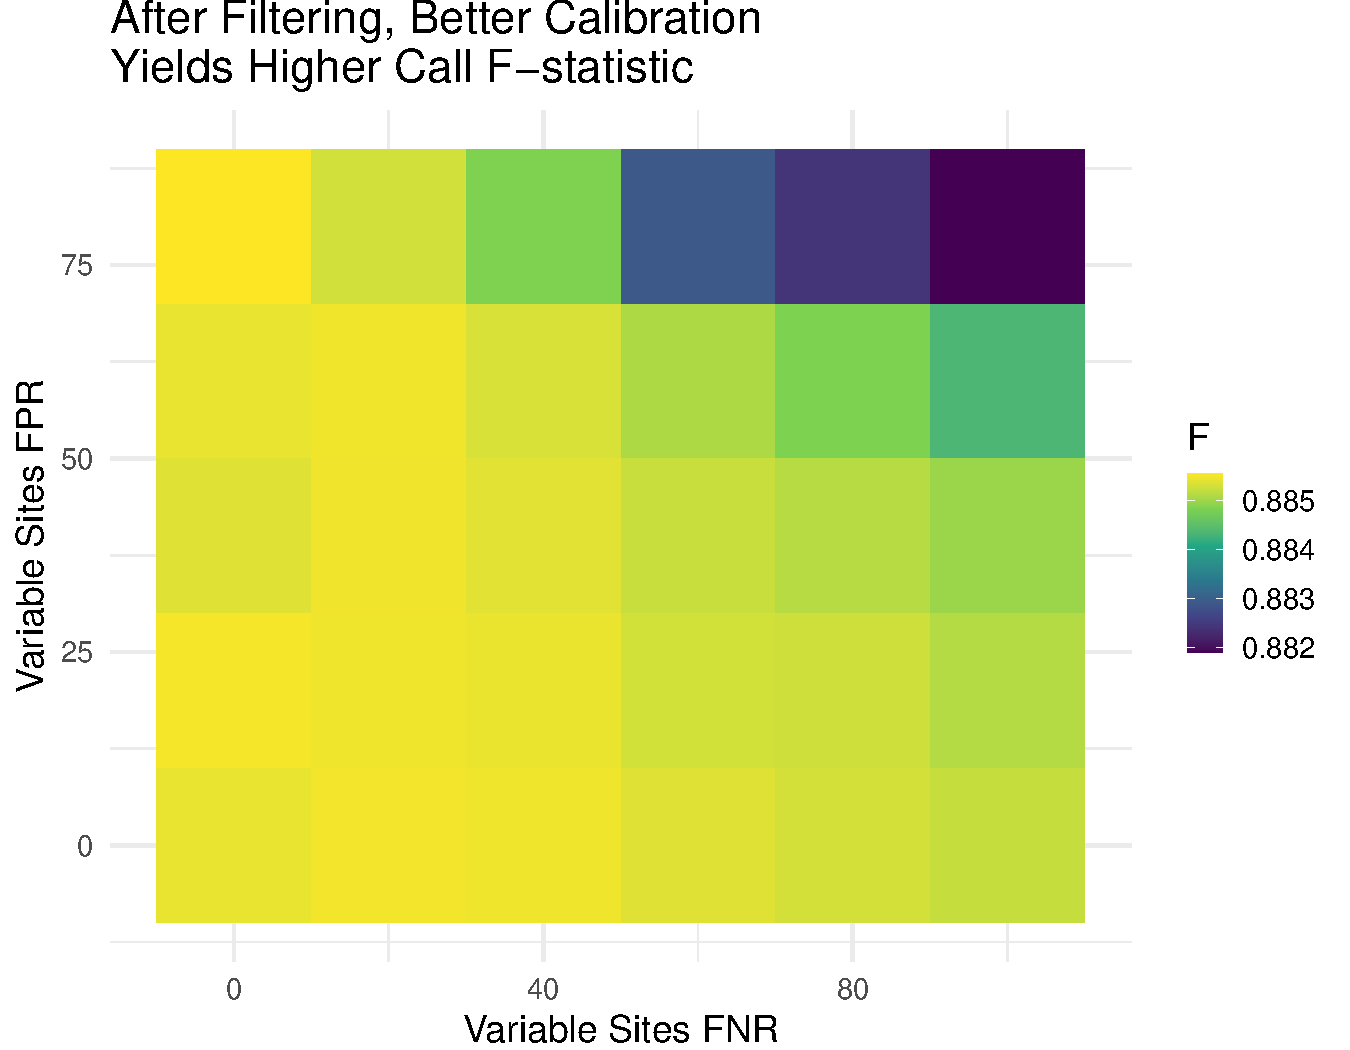
\includegraphics[width=.7\linewidth]{flt_f_heatmap.pdf}
\titlecaption{Filtered F-statistic}{The F-statistic of each dataset. As the calibration of the data improves, so does the F-statistic. This is in contrast to the unfiltered data, in which the worst-calibrated data has the best F-statistic. This difference is driven by an increase in relative precision of the best-calibrated data and a decrease in relative sensitivity of the poorly-calibrated data.}
\label{fig:vc_flt_f}
\end{figure}

%Simulated Reads results
Each of the three tested recalibration methods had only a small effect on the precision and sensitivity of HaplotypeCaller (see Figure \ref{fig:sim_sens_precision} and Table \ref{table:sim_summary}). The Initial-calls calibration did not change the precision compared to the raw quality scores, but did slightly decrease the sensitivity of the caller. GATK calibration using the true known variable sites yielded an increase in precision and sensitivity while the reference-free method KBBQ yielded an increase in precision but a slight decrease in sensitivity. Overall, this lead to an increase in the F-statistic after GATK recalibration with the true known sites and a decrease in the F-statistic after GATK recalibration with initial calls as the known sites, with no change in F-statistic after KBBQ recalibration. The ROC curve on the QUAL field of the called variants does not clearly show one calibration method as better than the others, and each one has the best trade-off between false positive and true positive rate at different points along the ROC curve except the Initial-calls calibration, which is closer to the bottom right of the plot at all times. There was no discernable difference between datasets when the GQ score was used to create the ROC curve, so it is not shown.

\begin{figure}
\centering
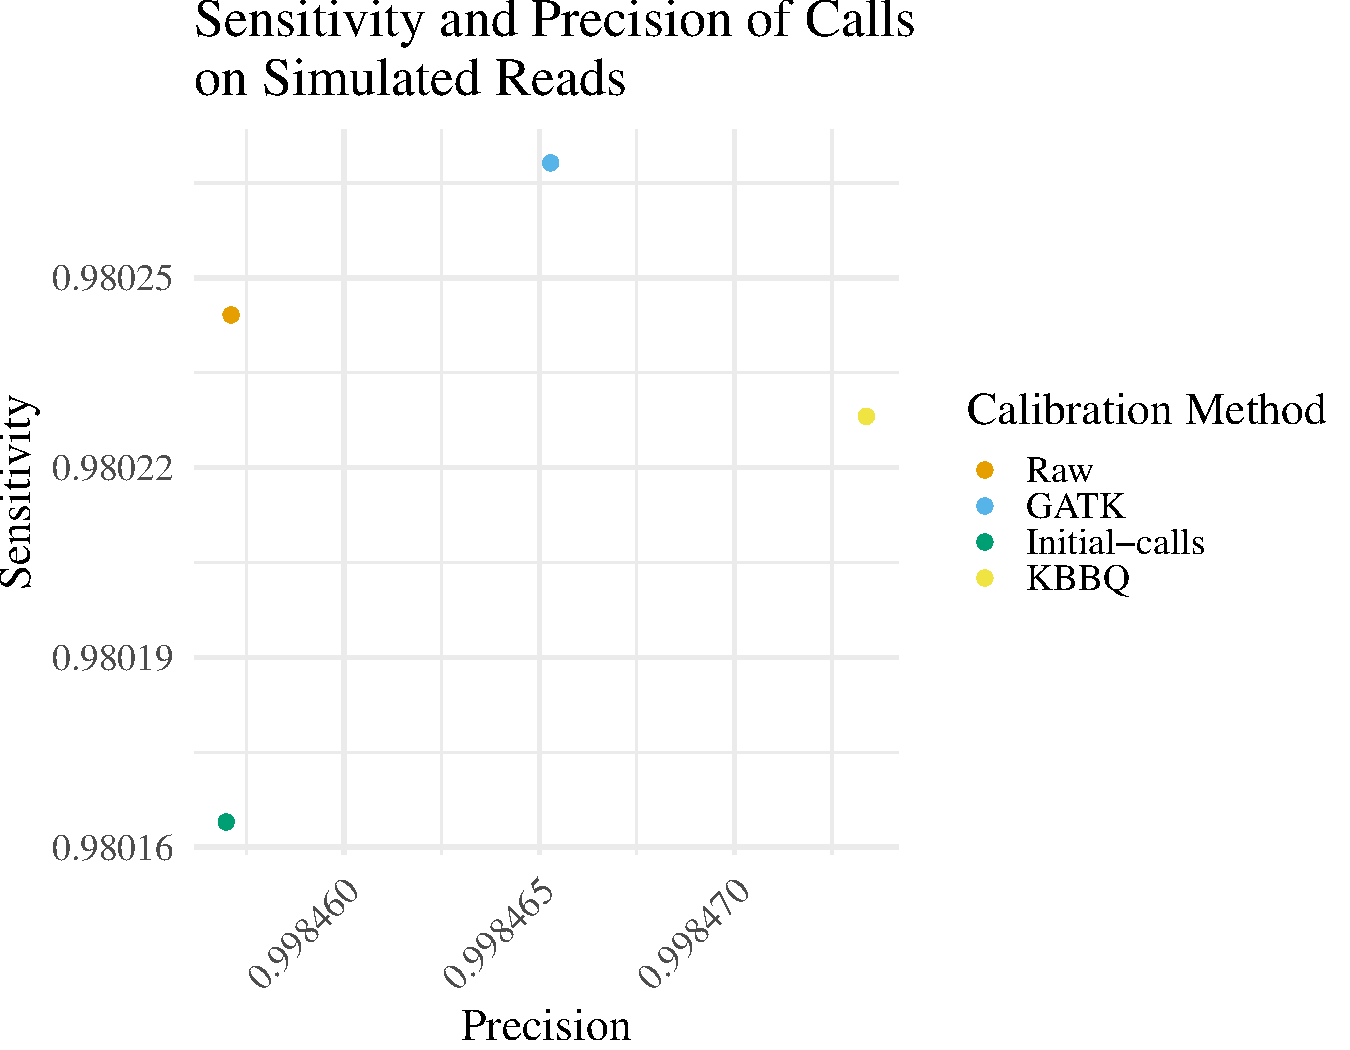
\includegraphics[width=.7\linewidth]{sims_sens_precision.pdf}
\titlecaption{Sensitivity and Precision of Calls on Simulated Reads}{The sensitivity and precision of calls made using the raw data and after recalibration with 3 methods. See Table \ref{table:sim_summary} for values plotted.}
\label{fig:sim_sens_precision}
\end{figure}

\begin{figure}
\centering
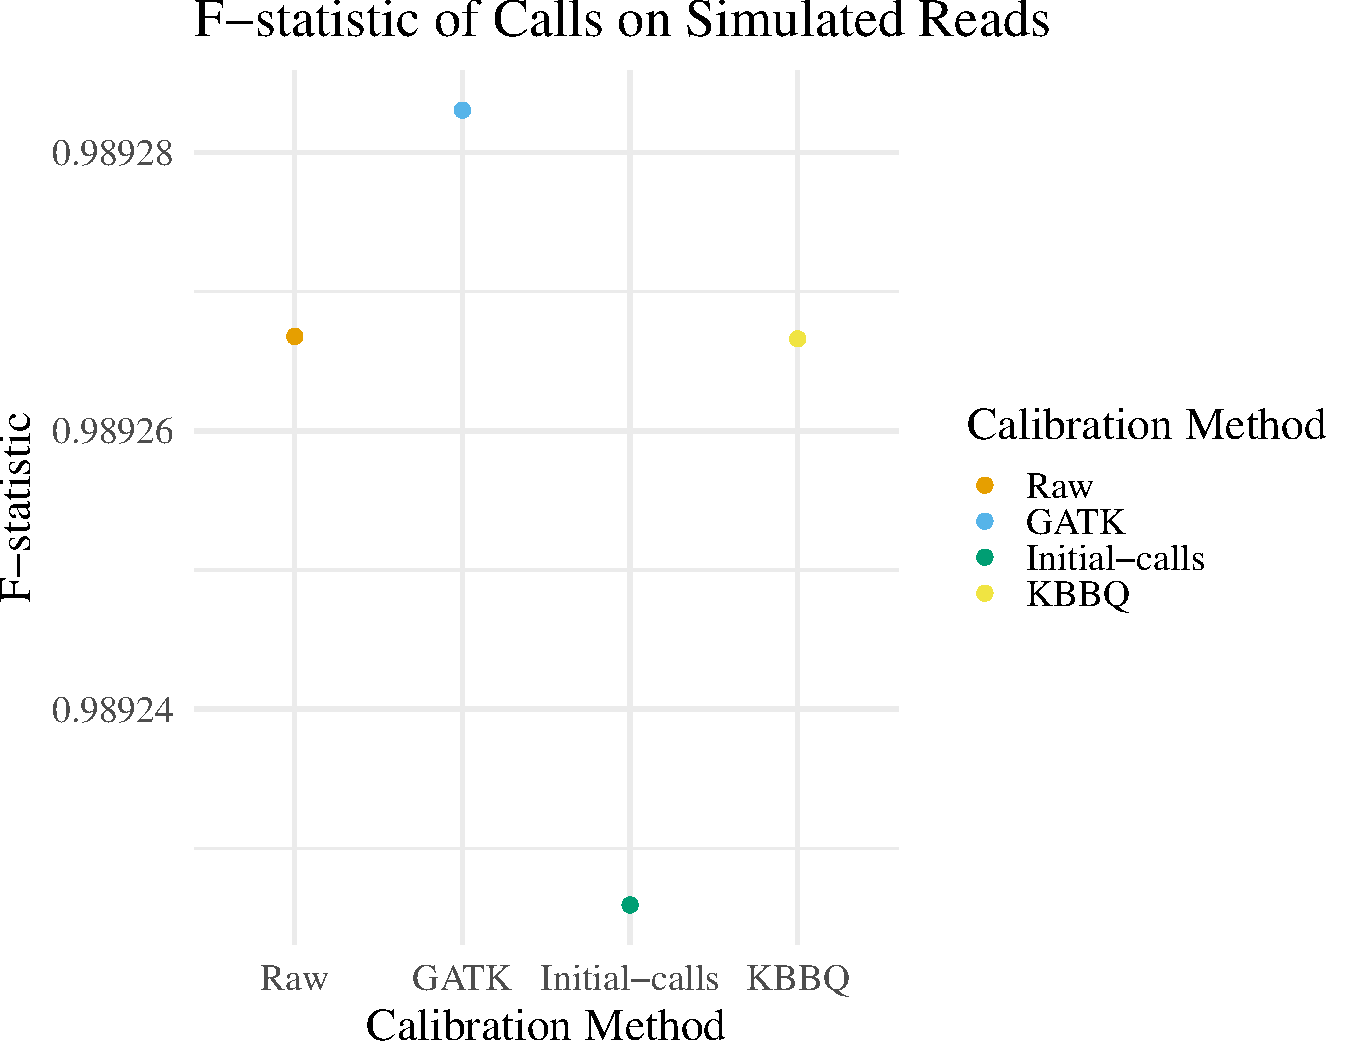
\includegraphics[width=.7\linewidth]{sims_fstat.pdf}
\titlecaption{F-statistic of Calls on Simulated Reads}{The F-statistic of calls made using the raw data and after recalibration with 3 methods. See Table \ref{table:sim_summary} for values plotted.}
\label{fig:sim_fstat}
\end{figure}

\begin{figure}
\centering
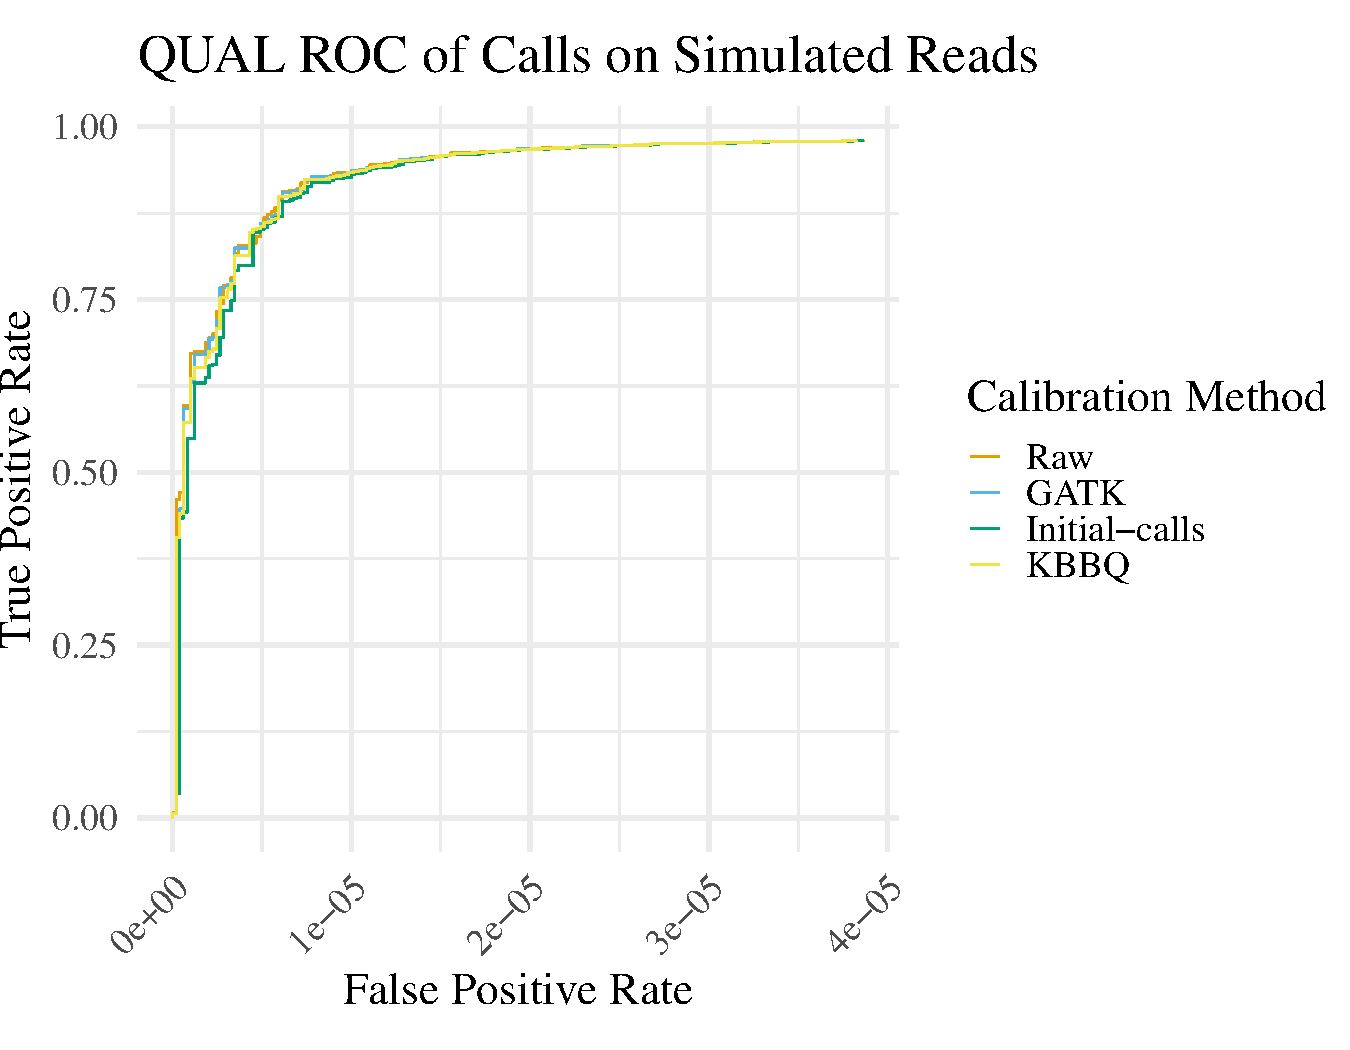
\includegraphics[width=.7\linewidth]{sims_qualroc.pdf}
\titlecaption{ROC of Calls on Simulated Reads}{ROC curve on the QUAL score of the variants called by HaplotypeCaller on the uncalibrated simulated reads and after recalibration with 3 methods.}
\label{fig:sim_qualroc}
\end{figure}


\begin{table}
\centering
\begin{tabular}{r l l l l l}
\toprule
Calibration Method & TP & FP & Sensitivity & Precision & F-statistic \\
\midrule
Raw & 122308 & 189 & 0.98024 & 0.99846 & 0.98927\\ 
GATK & 122311 & 188 & 0.98027 & 0.99847 & 0.98928\\ 
Initial-calls & 122298 & 189 & 0.98016 & 0.99846 & 0.98923\\ 
KBBQ & 122306 & 187 & 0.98023 & 0.99847 & 0.98927\\ 
\bottomrule
\end{tabular}
\titlecaption{Variant Caller Performance on Simulated Data}{A summary of the performance of HaplotypeCaller on simulated data calibrated different ways. TP is the number of true positive calls and FP the number of false positive calls. Raw is the quality scores assigned by the simulator, GATK is recalibration using the known heterozygous sites, Initial-calls is recalibration after calling an initial set of variants, and KBBQ is recalibration with the reference-free recalibrator KBBQ. See Figure \ref{fig:sim_sens_precision} for a visual comparison.}
\label{table:sim_summary}
\end{table}



\subsection{Variants Detected in \textit{E. melliodora}}

In order to determine the effect of reference-free recalibration on variant calls, I recalibrated the reads with the reference-free base quality score recalibrator KBBQ (see Chapter \ref{ch:kbbq} for more information on KBBQ). I then called variants and filtered the same way they were called and filtered in \textcite{orr_phylogenomic_2020}. The number of variants called at each step in the filtering process is shown in Table \ref{tbl:num_variants}. The number of variants called at each step using uncalibrated reads is shown in Table \ref{tbl:num_raw_variants}. After filtering, 106 variants were detected; 34 of these were also detected in the confident set of variants previously identified. This previous set had a total of 90 variants. Note that the number of detected sites listed in Table \ref{tbl:num_variants} are not all indicative of mutation, as the number includes heterozygous sites until the last filtering step.

\begin{table}
% \begin{tabularx}{\textwidth}{>{\hsize=1.5\hsize\linewidth=\hsize}X >{\hsize=.7\hsize\linewidth=\hsize}X >{\hsize=.9\hsize\linewidth=\hsize}X >{\hsize=.9\hsize\linewidth=\hsize}X}
\begin{tabularx}{\textwidth}{>{\hsize=1.5\hsize\linewidth=\hsize}X >{\hsize=.75\hsize\linewidth=\hsize}X >{\hsize=.75\hsize\linewidth=\hsize}X}
\toprule
\textbf{Description} & \textbf{Num.\newline{}Variants} & \textbf{Previously Identified Variants}\\
\midrule
Appears in first 11 scaffolds & 9838408 & 88\\
Total depth <= 500 & 9190223 & 87\\
ExcessHet <= 40 & 4932628 & 86\\
Not within 50bp of an indel & 3175128 & 69\\
Biallelic SNPs & 1913594 & 67\\
Outside repeat regions & 857810 & 46\\
All 3 replicates match & 63793 & 35\\
Only variable sites & 106 & 34\\
\bottomrule
\end{tabularx}
\titlecaption{Number of Detected Variants After KBBQ Recalibration}{The number of variants detected at each step in the filtering pipeline. Each row includes a description of each filter and the number of variants remaining after the filter has been applied. Previously identified variants are the number of variants that overlap the confident set described in \textcite{orr_phylogenomic_2020}. This set contains a total of 90 variants.}
\label{tbl:num_variants}
\end{table}

\begin{table}
\begin{tabularx}{\textwidth}{>{\hsize=1.5\hsize\linewidth=\hsize}X >{\hsize=.75\hsize\linewidth=\hsize}X >{\hsize=.75\hsize\linewidth=\hsize}X}
\toprule
\textbf{Description} & \textbf{Num.\newline{}Variants} & \textbf{Previously Identified Variants}\\
\midrule
Appears in first 11 scaffolds & 9823414 & 88\\
Total depth <= 500 & 9177547 & 87\\
ExcessHet <= 40 & 4924104 & 86\\
Not within 50bp of an indel & 3169769 & 69\\
Biallelic SNPs & 1911802 & 67\\
Outside repeat regions & 858383 & 46\\
All 3 replicates match & 63687 & 35\\
Only variable sites & 88 & 34\\
\bottomrule
\end{tabularx}
\titlecaption{Number of Detected Variants Using Uncalibrated Reads}{The number of variants detected at each step in the filtering pipeline using uncalibrated reads. See Table \ref{tbl:num_variants}.}
\label{tbl:num_raw_variants}
\end{table}

\section{Discussion}
\label{sec:kbbq_discussion}

These results show that GATK BaseRecalibrator is particularly vulnerable to false negatives (Figure \ref{figure:fnr}) in the database of variable sites, but is robust to false positives if the false negative rate is near 0 (Figure \ref{figure:fpr}). At the same time, when the false negative rate is not near 0, false positives will start to impact the calibration quality (Figure \ref{figure:fnrfpr}). Thus, when this database is unavailable and construction is required, it may be better to be liberal in deciding which sites may be variable to reduce the false negative rate as much as possible. This is in contrast to the GATK recommendation to use only the most confident sites when a database is unavailable.

The only rate that shows significant deviation from a 0\% false positive rate in the false-positive-only data is the 100\% false positive rate. Though a 100\% false positive rate with a 0\% false negative rate implies every site should be considered variable and ignored, the model curiously still has a source of errors it uses to recalibrate. Upon further investigation, this effect is driven by reads with alignments that begin with an insertion, as these inserted bases are not ignored by BaseRecalibrator when the first position of the site that should be ignored is equal to the first aligned position in the read. Thus, this line is a technical artifact. As long as there are enough bases available to analyze, the false positive rate doesn't significantly affect the performance of BaseRecalibrator at a false negative rate of 0. The calibrations of other datasets with a false positive rate of 100\% would also be affected by this artifact; however, in a real dataset it's unlikely to ever achieve a false positive rate of 100\%, so this artifact is unlikely to significantly affect real data.

%new para
Ultimately, if the false negative and false positive rates of the database of variable sites is high, GATK's procedure for BQSR \textit{can} cause miscalibration of the data worse than using raw quality scores, though this can only happen with very large error rates. In this dataset, the raw data has a RMSE of about 4, which is similar to a simulated dataset with a false negative rate between 40-60\% and a false positive rate between 60-80\%. In a real situation it's unlikely that error rates like this will occur, so BQSR will not severely destroy the input data. However, at even modest false negative and false positive error rates BQSR can cause undesirable miscalibration that could feasibly impact variants called from the data. Interestingly, at all error rates the calibration of quality scores below 25 is almost always correct or 1-off the true value. It seems that errors in the database of variable sites have a larger effect on higher quality predictions than lower ones.

Interestingly, overconfidence is not displayed in the reads recalibrated using the artificially constructed database of variable sites. This is likely because of how these variant sets were constructed; non-variable sites were selected independently and at random to be added to the set of purported variable sites. Thus a site containing an error and a site not containing an error are selected proportionally. In contrast, on a real dataset a variant calling algorithm would not make false positive errors independently; it is much more likely to classify a site as variable that has a sequencing error than to classify a site as variable that has no errors. That is: in this simulation, $P(\operatorname{classified\:positive} | \operatorname{actual\:negative})$ is independent of $P(\operatorname{sequencing\:error})$, but on an empirical dataset $P(\operatorname{classified\:positive} | \operatorname{actual\:negative})$ is likely not. Thus in reality false positives probably cause overconfidence in a similar manner that false negatives cause underconfidence.

Overall, these results show that as the quality of the calibration increases, the quality of the variant calls also slightly increases. The difference is very small, but better calibration produces more positive calls, with more true positive calls than any other recalibrated dataset. And though I only filtered the data with two fairly lenient filters, the best calibrations still produced the most true positive calls of any dataset except the calls made from data with the raw quality scores, which are not as well-calibrated (see Chapter \ref{ch:kbbq}) but produce more positive calls.

Interestingly, filtering seemed to amplify the difference between well-calibrated and poorly-calibrated data, increasing the disparity in the number of true positive variants detected. At the same time, filtering reduced the disparity in the number of false positive variants identified.

%Talk about how filtering becomes very important for leveraging the power of calibration
This observation makes filtering very important for variant calling. Variant callers generally prefer to include a putative variant rather than exclude it and miss a truly variant site. Thus, they prefer sensitivity over precision. The consequences of this preference can be seen in Figure \ref{fig:vc_sens_prec}, where filtering reduced the sensitivity of every set of calls but greatly improved precision and decreased the precision disparity between datasets. Filtering raw calls is paramount to getting a variant set with acceptable levels of sensitivity and precision. Ultimately, the impact of base quality score recalibration is not as large as the filters one chooses to use. In this case, better calibration results in an increased precision of .007 before filtering; filtering itself increased precision by about .014, while reducing sensitivity by approximately .18. So the effect of calibration on sensitivity and precision is small in comparison to the effect of filtering. At the same time, important variants that matter for the purposes of the study being conducted could be missed, so this difference in calibration could be relevant.

Unfortunately, this means that filtering plays a big role in the success of a variant calling pipeline. While there is no definitive best way to filter variants in all cases, Figure \ref{fig:vc_rocs} shows that differences in quality score calibration can affect the annotations attached to each call and make the same filters more or less effective, depending on the threshold used. While this is interesting, it doesn't necessarily change how filtering should be done or suggest an optimal filtering strategy.

One limitation of this study is that it uses only a sparse range of false positives and false negatives in the database of variable sites. Especially since the effect of calibration on the output variant calls is small, a different dataset may yield different results. As seen in Chapter \ref{ch:kbbq}, the calibration of the raw reads in this dataset is not particularly bad, though it is worse than all other datasets. Replication with other datasets and other variant callers is necessary to further elucidate the role of base quality score calibration on variant caller performance.

Furthermore, the CHM1-CHM13 data is from a human-derived cell line, and protocols for DNA extraction and sequencing are fairly well-established. Additionally, the original base calling algorithm is likely tuned to work well with human-like data. All together, this means that while the effect of recalibration was not particularly pronounced in this dataset, base quality score recalibration may have a higher impact on data that is messier, contains more errors induced in sample preparation, or results from failed sequencing runs. In light of this, it seems that using the default-assigned base quality scores will offer superior performance unless one has a reason to suspect the data is of poor quality.

% Simulated Data
% Each of the three tested recalibration methods had only a small effect on the precision and sensitivity of HaplotypeCaller (see Figure \ref{fig:sim_sens_precision} and Table \ref{table:sim_summary}). The Initial-calls calibration did not change the precision compared to the raw quality scores, but did slightly decrease the sensitivity of the caller. GATK calibration using the true known variable sites yielded an increase in precision and sensitivity while the reference-free method KBBQ yielded an increase in precision but a slight decrease in sensitivity. Overall, this lead to an increase in the F-statistic after GATK recalibration with the true known sites and a decrease in the F-statistic after GATK recalibration with initial calls as the known sites, with no change in F-statistic after KBBQ recalibration. The ROC curve on the QUAL field of the called variants does not clearly show one calibration method as better than the others, and each one has the best trade-off between false positive and true positive rate at different points along the ROC curve except the Initial-calls calibration, which is closer to the bottom right of the plot at all times. There was no discernable difference between datasets when the GQ score was used to create the ROC curve, so it is not shown.

The simulated reads similarly show that the effect of base quality score recalibration is fairly small. However, the simulator also assigned fairly well-calibrated scores to begin with, so there is not much room for improvement in those scores and many opportunities to make calibration worse. As shown in the previous chapter, using initial calls for recalibration does degrade the overall quality of the calibration. This is consistent with these results showing that HaplotypeCaller performs worse on reads recalibrated using GATK with a set of initial calls. However, when the set of known sites is the true set of variable sites in the data, GATK recalibration does slightly improve the precision and sensitivity of HaplotypeCaller. At the same time, reference-free recalibration with KBBQ increases precision but slightly decreases sensitivity.

Overall, these simulations show that GATK recalibration slightly increases HaplotypeCaller performance if the set of variable sites is complete and has no false positives, even if the starting data is fairly well-calibrated. However, if the set of variable sites is not complete, GATK recalibration will cause HaplotypeCaller performance to suffer slightly. Thus, if there is a risk that the set of variable sites is inaccurate, GATK recalibration should not be used. At the same time, raw quality scores will provide good performance as long as they are fairly well-calibrated to start. These simulations also show that even with well-calibrated input data, the reference-free recalibration method KBBQ doesn't significantly degrade the performance of HaplotypeCaller.

%



%Speculate about when BQSR might actually be useful!! More work is needeD!!!

% Surprisingly, the behavior of the raw dataset is most similar to that of KBBQ and the dataset calibrated with perfect information. At the same time, the patterns observed clearly indicate an effect of calibration on how HaplotypeCaller functions. This can be explained in a few ways; 1) GATK's own calibration method is flawed, and the raw data is truly the best calibrated data, so the trends are real. 2) this dataset is just weird 3) the calibration is actually correct and calibration affects HC in a roundabout way that doesn't directly translate into better calls. The trends are an artifact of that process.

\subsection{KBBQ Recalibration Yielded More \textit{E. melliodora} Calls}

While the simulated datasets revealed a complex interaction between the number of detected variants, sensitivity, precision, and filtering, it appears KBBQ recalibration improved the ability to successfully call variants in a non-model organism. In Chapter \ref{ch:kbbq}, I showed that using GATK's recommended approach of calling confident variants and using those as the set of variable sites to use in recalibration results in poor base quality score calibration. I also showed that using KBBQ improved calibration to be comparable to GATK recalibrations with perfect information. The calls on the simulated datasets shown here also imply that KBBQ recalibrated reads behave similarly to or better than reads recalibrated with GATK using perfect information.

Using the same calling and filtering parameters as those used in \textcite{orr_phylogenomic_2020} yielded more variants at the end of filtering with 106 instead of 99. This is consistent with the results from the simulated datasets, where better-calibrated data yields more variant calls. It is also consistent with \textcite{ni_improvement_2016}, who find that better calibration increases sensitivity. Indeed, this is the case even before other filters are applied, with 9,838,408 variants detected versus 9,679,544 detected in the prior study. This is also slightly more than the 9,823,414 detected using uncalibrated reads before filtering and 88 detected after.

Additionally, the number of variants after filtering that appear in the confident set identified in the previous study increased from 30 to 34. This is identical to the number detected using the raw reads. Thus, using KBBQ to recalibrate the reads before calling seems to have increased the sensitivity of the variant calling pipeline compared to GATK's BaseRecalibrator. Note that the confident call set in \textcite{orr_phylogenomic_2020} has a fairly large estimated false negative rate of approximately 30\% and many reads did not map to the genome used; thus, it's likely there are many additional true variants in the data that were not previously identified but are nevertheless true variants.

\section{Conclusion}

The simulated data here shows that quality scores do have a small but important effect on the quality of the called variants. This manifests itself in not only the difference in the number of true positive calls and the number of false positive calls, but also in the QUAL and GQ annotations. The simulated data suggest the size of the effect is small, but on an empirical dataset increased calibration yielded a substantial number of additional variants. While effective recalibration will certainly benefit variant calling, these results show BaseRecalibrator can decrease the quality of the called variants if done improperly. If very high sensitivity is critical to the analysis being performed, care must be taken to ensure that base quality scores are properly calibrated.

\printbibliography[segment=\therefsegment]{}
